%%%%%%%%%%%%%%%%%%%% manuscript.tex %%%%%%%%%%%%%%%%%%%%%%%%%%%%%%%%%%%
% ICICCDS 2027 contribution -- Peruvian Altiplano streamflow ML
% Springer SVMult template (contributed volume style)
%%%%%%%%%%%%%%%%%%%%%%%%%%%%%%%%%%%%%%%%%%%%%%%%%%%%%%%%%%%%%%%%%%%%%%%

\documentclass[graybox]{svmult}

\usepackage{mathptmx}
\usepackage{helvet}
\usepackage{courier}
\usepackage{graphicx}
\usepackage{multicol}
\usepackage[bottom]{footmisc}
\usepackage{booktabs}
\usepackage{amsmath}
\usepackage{url}
\usepackage{natbib}

\graphicspath{{figuras/}{../../04-resultados/figuras/}}

\begin{document}

\title*{Open-data machine learning for streamflow and hydrological drought forecasting in the Peruvian Altiplano}
\titlerunning{Open-data ML for Altiplano streamflow forecasting}

\author{Richar Andre Vilca-Solorzano and Dina Maribel Yana-Yucra}
\authorrunning{Vilca-Solorzano and Yana-Yucra}

\institute{Richar Andre Vilca-Solorzano \at Universidad Nacional del Altiplano, Puno, Peru \\
\email{avilca@unap.edu.pe}
\and
Dina Maribel Yana-Yucra \at Universidad Nacional del Altiplano, Puno, Peru}

\maketitle

\abstract*{Hydrological drought and highly variable streamflow threaten water security across the Peruvian Altiplano. We present a fully open, reproducible machine-learning pipeline for short-horizon streamflow forecasting and a simple hydrological drought index using publicly available discharge and climate series. On the SENAMHI gauge Puente Isla Cabanillas (Andean-GC open release), 1-day persistence remains strongest (NSE~$0.907$), while Ridge regression improves 7-day forecasts over persistence (NSE~$0.562$ vs.\ $0.486$; skill $+0.077$). All data URLs, licenses, code, and metrics are released with the paper.}

\abstract{Hydrological drought and highly variable streamflow threaten water security for communities and agriculture across the Peruvian Altiplano. Operational forecasting is often limited by sparse gauges and uneven access to proprietary models. We present a fully open, reproducible machine-learning pipeline for short-horizon streamflow forecasting and hydrological drought indication using publicly available discharge and climate series for an Altiplano basin. After quality control and lag-based feature construction, we compare classical baselines (persistence and seasonal climatology) against lightweight learners suitable for commodity laptops (Ridge, random forests, gradient boosting, XGBoost, and a small MLP), under a strict temporal train--validation--test split that prevents leakage. On the SENAMHI gauge Puente Isla Cabanillas (Andean-GC QC series, 2000--2024 analysis window), 1-day persistence achieves the highest test NSE ($0.907$); ML models reach NSE~$0.85$--$0.87$ but do not beat persistence at lead~1. At lead~7 days, Ridge improves upon persistence (NSE~$0.562$ vs.\ $0.486$; skill vs.\ persistence $+0.077$). We further derive a month-standardized 30-day streamflow index (SSI-like) for early-warning illustration. The study does not claim operational replacement of national hydrological services; it offers a transparent benchmark for data-sparse Andean catchments.}

\section{Introduction}
\label{sec:intro}
The Peruvian Altiplano, including tributaries of Lake Titicaca in the Puno region, experiences strong wet--dry seasonality and recurrent hydrological stress. Open gauges and climate reanalyses now enable transparent machine-learning (ML) benchmarks that can be reproduced on a laptop, complementing national services without requiring proprietary stacks~\cite{kratzert2019lstm}.

This contribution asks whether lightweight ML models improve short-horizon streamflow forecasts over naive baselines when trained only on open data for an Altiplano gauge, and whether a simple standardized streamflow index can be derived from the same series for drought indication.

\section{Data and study area}
\label{sec:data}
We use quality-controlled daily discharge from the Andean Glacierized Catchment (Andean-GC) dataset~\cite{aguayo2026andeangc}, which redistributes institutional records under an open Zenodo release (CC~BY~4.0). The primary station is SENAMHI gauge \textbf{Puente Isla Cabanillas} (Andean-GC id \texttt{P00000055}; $15.4721^\circ$\,S, $70.2244^\circ$\,W; basin area $\approx 2843$\,km$^2$), a tributary system contributing to Lake Titicaca via the Cabanillas--Coata pathway. The QC series spans 1994-07-16 to 2024-12-31 ($n=6572$ daily values; mean discharge $22.86$\,m$^3$\,s$^{-1}$).

Daily precipitation at the gauge coordinates was obtained from the Open-Meteo Historical Weather API~\cite{openmeteo}, which serves ERA5-Land-based fields~\cite{era5land}, for 2000-01-01 to 2024-12-31. The multivariate experiment uses the 2000--2024 overlap ($n=5854$ discharge days). Official ANA/SNIRH portals and a HydroShare Peru discharge bag were probed but were not downloadable in batch within the submission window (HTTP 404 / request-based access); documentation of all attempted URLs and licenses is in the repository file \texttt{02-datos/fuentes/INVENTARIO.md}.

\begin{figure}[htbp]
\centering
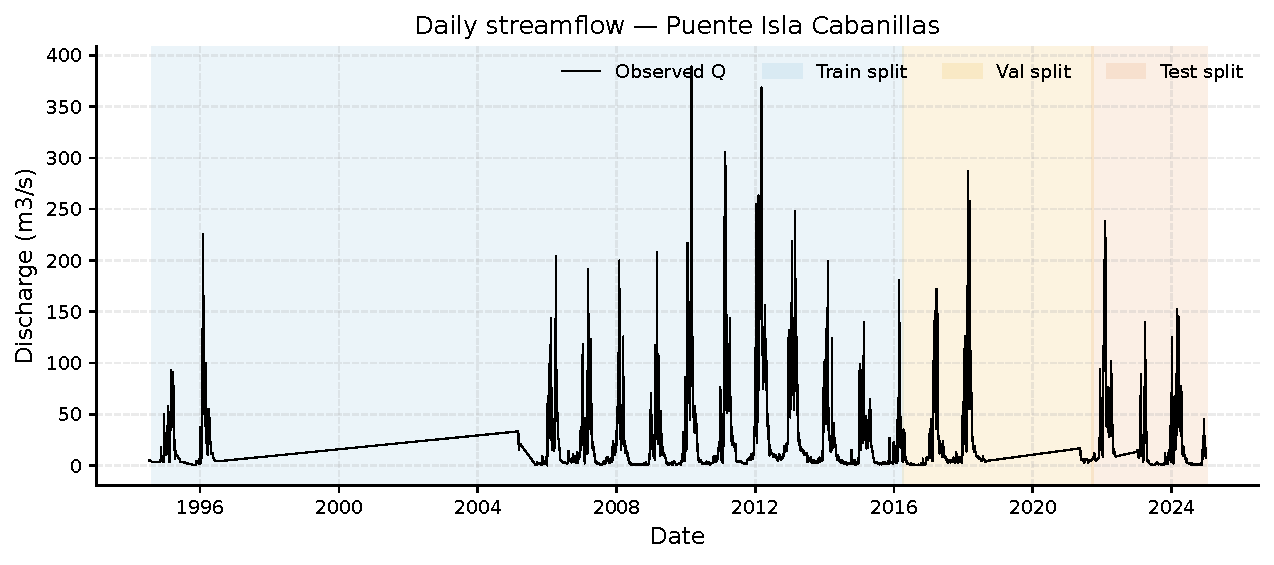
\includegraphics[width=0.95\textwidth]{fig01_hydrograph_cabanillas.pdf}
\caption{Daily discharge at Puente Isla Cabanillas with chronological train, validation, and test partitions (lead-1 feature table).}
\label{fig:hydro}
\end{figure}

\section{Methods}
\label{sec:methods}
\subsection{Features and split}
For forecast horizons $h\in\{1,7\}$ days we build lag features of discharge ($1,2,3,7,14,30$\,d), rolling means/standard deviations ($7,14,30$\,d, shifted to avoid leakage), precipitation lags and rolling sums, and Fourier seasonality terms ($\sin/\cos$ of day-of-year). The target is $Q_{t+h}$. Persistence uses $Q_t$ as the forecast of $Q_{t+h}$; climatology uses the training-period day-of-year mean smoothed with a 7-day circular window.

Rows with missing features or targets are dropped. Remaining samples are split \textbf{chronologically} into 70\% train / 15\% validation / 15\% test (no shuffling). Models are fit on train only; metrics are reported exclusively on the held-out test period. For lead~1 the test window contains $n=874$ days.

\subsection{Models}
Baselines: persistence and seasonal climatology. Learners: Ridge regression (standardized features), Random Forest (200 trees), Gradient Boosting (200 trees), XGBoost (300 trees), and a small MLP ($64$--$32$ hidden units) with early stopping. All runs used a laptop CPU; total training wall time was under one minute for the full suite.

\subsection{Metrics}
We report RMSE, MAE, Nash--Sutcliffe efficiency (NSE)~\cite{nash1970river}, and skill versus persistence:
\begin{equation}
\mathrm{skill}=1-\frac{\mathrm{RMSE}_{\mathrm{model}}}{\mathrm{RMSE}_{\mathrm{persistence}}}.
\end{equation}
Positive skill indicates improvement over persistence.

\subsection{Drought index}
Following the spirit of standardized indices~\cite{mckee1993spi}, we compute a 30-day mean discharge and standardize by calendar month (approximate SSI-30) for exploratory drought visualization (Fig.~\ref{fig:ssi}).

\section{Results}
\label{sec:results}
Table~\ref{tab:metrics} summarizes test metrics. At lead~1\,d, \textbf{persistence is best} (NSE~$0.907$, RMSE~$11.30$\,m$^3$\,s$^{-1}$). Among ML models, the MLP attains the highest NSE ($0.871$) but still underperforms persistence (skill $-0.176$). This is expected when day-to-day autocorrelation dominates.

At lead~7\,d, autocorrelation weakens: Ridge achieves NSE~$0.562$ and skill $+0.077$ versus persistence (NSE~$0.486$), with MLP close (NSE~$0.559$, skill $+0.073$). Tree ensembles underperform Ridge at this horizon on this station, suggesting that linear combinations of lagged $Q$ and seasonal terms already capture much of the predictable signal.

\begin{table}[htbp]
\centering
\caption{Test-set metrics for Puente Isla Cabanillas (real run; chronological split).}
\label{tab:metrics}
\begin{tabular}{llrrrr}
\toprule
Model & $h$ (d) & RMSE & MAE & NSE & Skill vs pers. \\
\midrule
persistence & 1 & 11.30 & 4.76 & 0.907 & 0.000 \\
climatology & 1 & 30.33 & 17.25 & 0.327 & $-1.685$ \\
Ridge & 1 & 14.15 & 8.18 & 0.854 & $-0.252$ \\
RandomForest & 1 & 13.91 & 6.72 & 0.858 & $-0.231$ \\
GradientBoosting & 1 & 13.85 & 7.02 & 0.860 & $-0.226$ \\
MLP & 1 & 13.28 & 6.97 & 0.871 & $-0.176$ \\
XGBoost & 1 & 14.10 & 7.01 & 0.854 & $-0.248$ \\
\midrule
persistence & 7 & 26.50 & 12.71 & 0.486 & 0.000 \\
climatology & 7 & 30.22 & 17.09 & 0.331 & $-0.141$ \\
Ridge & 7 & 24.45 & 14.91 & 0.562 & $+0.077$ \\
RandomForest & 7 & 28.17 & 15.31 & 0.419 & $-0.063$ \\
GradientBoosting & 7 & 28.42 & 15.42 & 0.408 & $-0.073$ \\
MLP & 7 & 24.55 & 13.76 & 0.559 & $+0.073$ \\
XGBoost & 7 & 29.45 & 15.81 & 0.365 & $-0.111$ \\
\bottomrule
\end{tabular}
\end{table}

\begin{figure}[htbp]
\centering
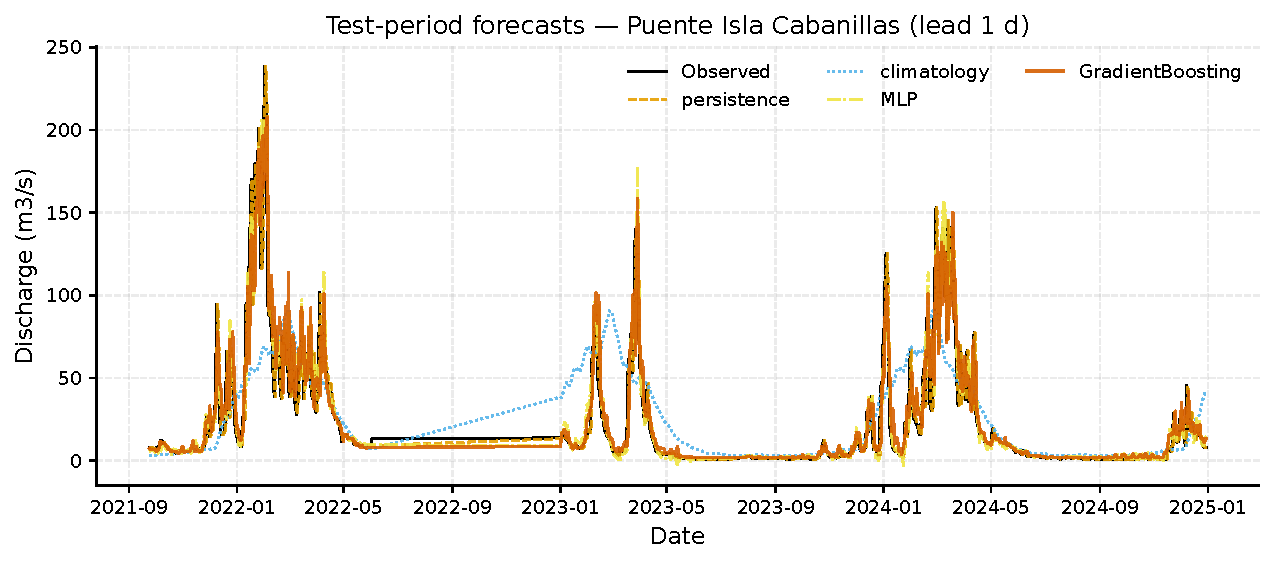
\includegraphics[width=0.95\textwidth]{fig02_forecast_test_h1.pdf}
\caption{Test-period forecasts at lead 1 day versus observations.}
\label{fig:fc1}
\end{figure}

\begin{figure}[htbp]
\centering
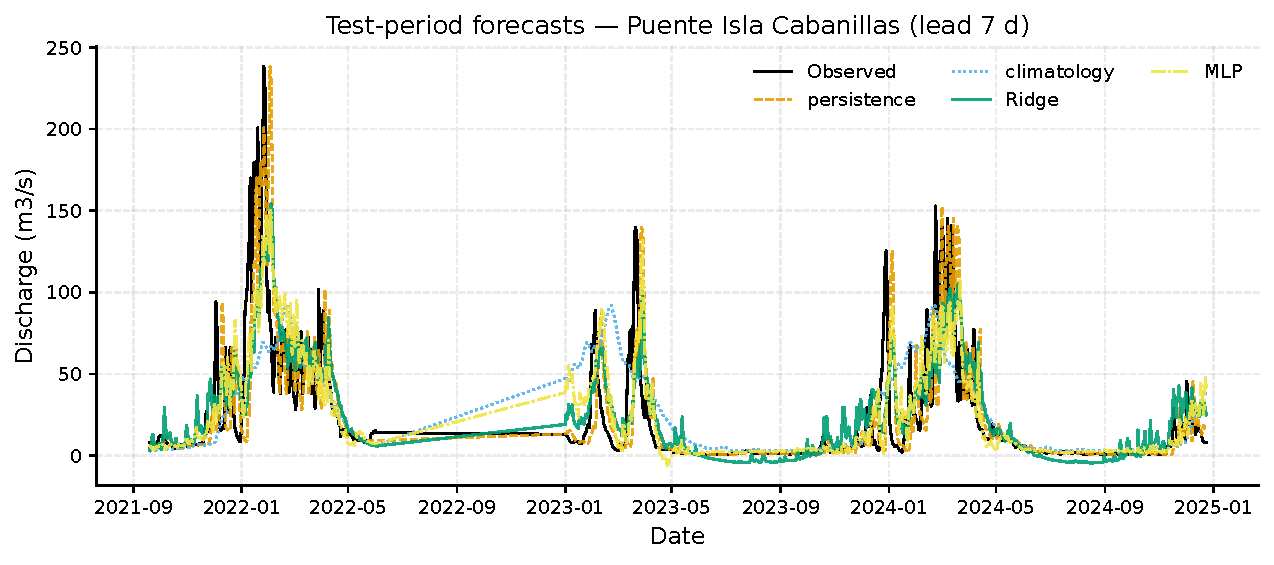
\includegraphics[width=0.95\textwidth]{fig02_forecast_test_h7.pdf}
\caption{Test-period forecasts at lead 7 days versus observations.}
\label{fig:fc7}
\end{figure}

\begin{figure}[htbp]
\centering
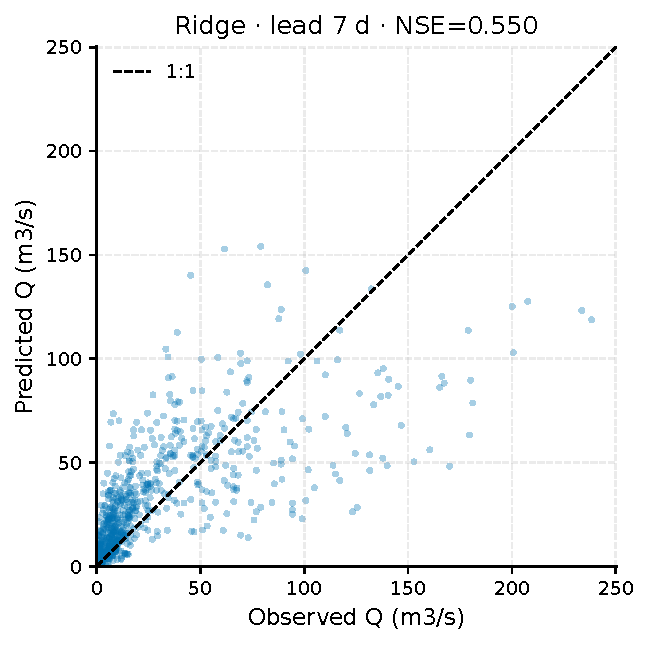
\includegraphics[width=0.72\textwidth]{fig03_scatter_best_h7.pdf}
\caption{Observed versus predicted discharge on the test set for the best ML model at lead 7 days (Ridge, NSE~$0.562$).}
\label{fig:scatter}
\end{figure}

\begin{figure}[htbp]
\centering
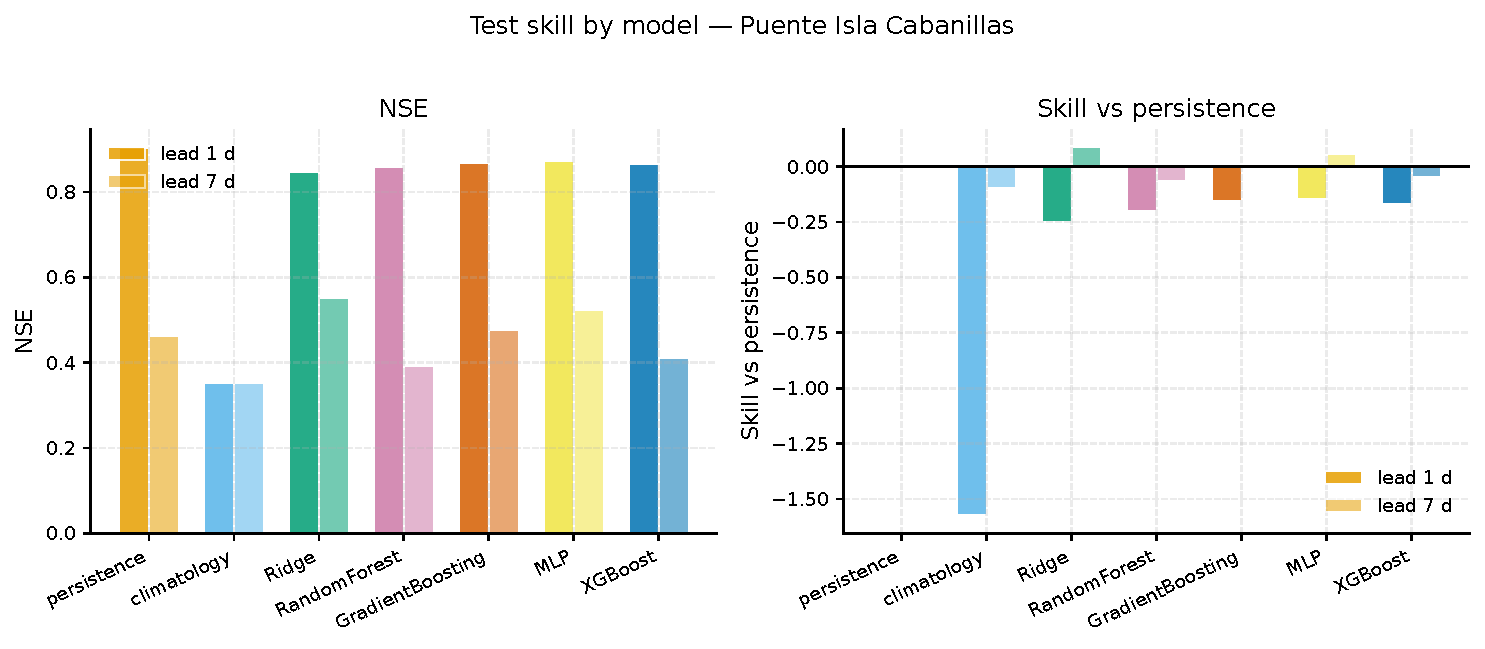
\includegraphics[width=0.95\textwidth]{fig04_skill_bars.pdf}
\caption{Test NSE and skill versus persistence by model and horizon.}
\label{fig:skill}
\end{figure}

\begin{figure}[htbp]
\centering
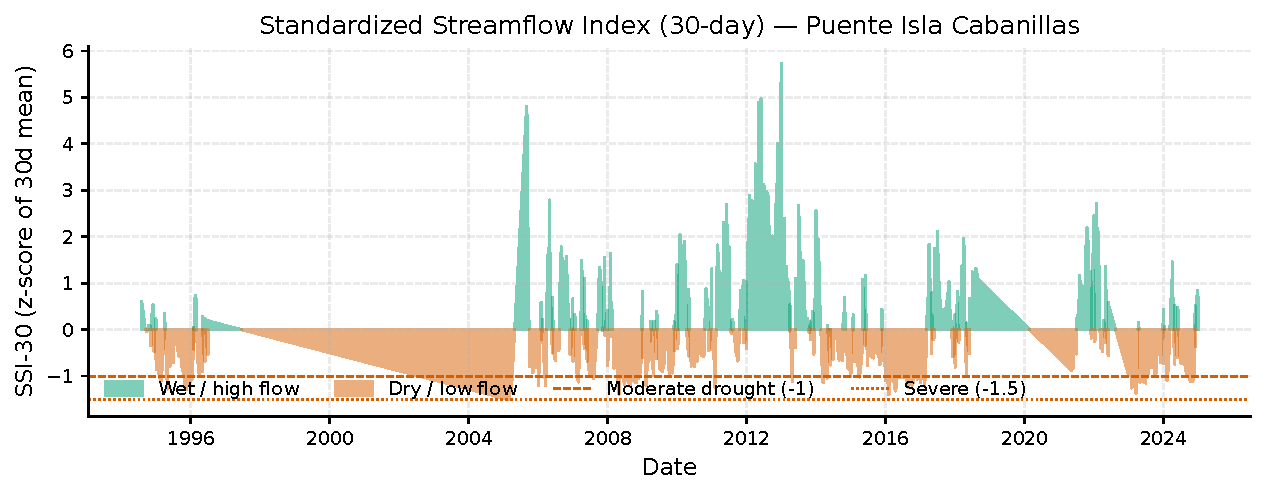
\includegraphics[width=0.95\textwidth]{fig05_ssi30.pdf}
\caption{Approximate month-standardized 30-day streamflow index (SSI-30) at Puente Isla Cabanillas.}
\label{fig:ssi}
\end{figure}

\section{Discussion and limitations}
\label{sec:limits}
Strong 1-day persistence skill implies that claiming ``ML superiority'' without baseline comparison would be misleading; honest reporting is itself a contribution for Andean open-data studies. Gains at 7 days from Ridge/MLP are modest but positive and obtained without deep learning or cloud GPUs.

Limitations include: (i) a single primary gauge (Salcca was extracted but too short for the same protocol); (ii) precipitation from reanalysis rather than local SENAMHI pluviometers; (iii) SSI approximated by monthly $z$-scores rather than a full parametric SPI/SSI fit; (iv) no spatial multi-basin transfer learning; (v) simulated national products (e.g., PISCO-ARNOVIC) were not used as ground truth. Results are not an operational forecast product.

\section{Conclusions}
\label{sec:concl}
We released a complete open-data ML study for Altiplano streamflow forecasting centered on Puente Isla Cabanillas. Persistence dominates at 1-day lead; Ridge and a small MLP improve 7-day forecasts over persistence. Code, processed tables, 600\,dpi figures, and a source inventory accompany the manuscript to support reproduction and extension to additional Titicaca tributaries (Ramis, Ilave, Coata, Huancan\'e) when further open gauges become available.

\begin{acknowledgement}
The authors thank open-data providers Andean-GC/Zenodo, SENAMHI (institutional source of the redistributed gauge), and Open-Meteo/Copernicus. Computations were performed on a laptop CPU only.
\end{acknowledgement}

%% Alternative if acknowledgement env unavailable:
% \section*{Acknowledgements}
% ...

\bibliographystyle{spbasic}
\bibliography{references}

\end{document}
